%%%%%%%%%%%%%%%%%%%%%%%%%%%%%%%%%%%%%%%%%%%%%%%%%%%%%%%%%%%%%%%%%%%%%%%
%% Trim Size: 9.75in x 6.5in
%% Text Area: 8in (include Runningheads) x 5in
%% ws-acs.tex   :   7-5-2008
%% Tex file to use with ws-acs.cls written in Latex2E.
%% The content, structure, format and layout of this style file is the
%% property of World Scientific Publishing Co. Pte. Ltd.
%% Copyright 1995, 2002 by World Scientific Publishing Co.
%% All rights are reserved.
%%%%%%%%%%%%%%%%%%%%%%%%%%%%%%%%%%%%%%%%%%%%%%%%%%%%%%%%%%%%%%%%%%%%%%%
%
%%%%%%%%% FOR TEMPLATE OF TYPING OUT THE BIBLIOGRAPHY TEXT ONLY %%%%%%%%
\newcounter{myctr}
\def\myitem{\refstepcounter{myctr}\bibfont\parindent0pt\hangindent15pt[\themyctr]\enskip}
\def\myhead#1{\vskip10pt\noindent{\bibfont #1:}\vskip4pt}
%%%%%%%%% FOR TEMPLATE OF TYPING OUT THE BIBLIOGRAPHY TEXT ONLY %%%%%%%%

\documentclass{ws-acs}
\usepackage{url}
\usepackage{cite}
\begin{document}

\makeatletter
\def\@biblabel#1{[#1]}
\makeatother

\markboth{Rocco Paolillo and Jan Lorenz}{How different homophily preferences mitigate and spur ethnic and value segregation: Schelling's model extended}

%%%%%%%%%%%%%%%%%%%%% Publisher's Area please ignore %%%%%%%%%%%%%%%
%
\catchline{}{}{}{}{}
%
%%%%%%%%%%%%%%%%%%%%%%%%%%%%%%%%%%%%%%%%%%%%%%%%%%%%%%%%%%%%%%%%%%%%

\title{HOW DIFFERENT HOMOPHILY PREFERENCES MITIGATE AND SPUR ETHNIC AND  VALUE  SEGREGATION: SCHELLING'S MODEL EXTENDED}

\author{ROCCO PAOLILLO}

\address{Bremen International Graduate School of Social Sciences, Jacobs University Bremen \& University of Bremen, \\
Campus Ring 1,
Bremen, 28759,
Germany\\
rpaolillo@bigsss-bremen.de}

\author{JAN LORENZ}

\address{Bremen International Graduate School of Social Sciences, Jacobs University Bremen\\ Campus Ring 1
Bremen, 28759,
Germany\\
j.lorenz@jacobs-university.de}

\maketitle

\begin{history}
\received{(received date)}
\revised{(revised date)}
%\accepted{(Day Month Year)}
%\comby{(xxxxxxxxxx)}
\end{history}

\begin{abstract}
In Schelling's model of segregation agents of two ethnicities live in a regular grid and aim at staying in a neighborhood with at least a certain fraction of same ethnicity. The model demonstrates how even small thresholds of desired fractions at local level of individuals can cause emergence of high degree of segregation at the societal level. Nevertheless, similarity based on a dichotomous and exhaustive definition of ethnicity and lack of mechanisms of integration, might hinder the contributions of the model for modern and multicultural societies. In multicultural societies shared tolerance towards diversity is likely to play a significant role in defining similarity between people also within ethnic groups and affect the patterns of segregation/integration in society. Bearing this in mind, we added to the original ethnicity-oriented homophily of agents, a value-oriented subpopulation of tolerant agents. In our experiments we observe what profile of value and ethnic segregation emerge from the combination of value similarity and ethnic similarity threshold of the two types of agents in equal group size and majority/minority conditions. Our results show how the introduction of value-oriented similarity reduces the ethnic segregation of the original model and a spillover effect emerges for which value segregation favor under some constraints ethnic segregation.
\end{abstract}

\keywords{Schelling model; segregation; tolerance.}

\section{Introduction}
We all live in societies where we are connected with other people. Societies today are characterized by increasing diversity, due to migration flow and coexistence of people belonging to different cultures and ethnic background. Spatial segregation referred to as the distribution in space of different groups across neighborhoods of a city \cite{clark2015} is a critical issue, often considered as the result of the active intention to not integrate with people of other groups \cite{clark2008}. Schelling's model \cite{schelling69} demonstrates on the contrary how segregation can be the emerging result of people preferring to live close to those considered as similar regardless of any negative orientation towards others. Adopting a complex systems perspective, in Schelling's model segregation emerges from mutual adaptation of people following the own homophily preferences under spatial proximity constraints.  The model shows that dramatic levels of segregation could emerge even from small degrees of homophily preferences of individuals. Limits that could be addressed to Schelling's model is to consider similarity between people as built on an unique, exclusive dimension as ethnicity and focus on the convergence towards segregation. This is likely to not represent the complexity of modern and multicultural societies where segregation where integration between diverse groups is more desired and promotion of tolerance adovated \cite{verkuyten2010}. Bearing this idea in mind, we extended Schelling's model by introducing a differentiation in the homophily behavior of agents based on ethnicity-oriented and value-oriented similaity. In our simulations we observe what profiles of societal segregation emerge in stylized scenarios from the mutual adaptation of these two types of agents in an equa group size and majority/minority condition.

The goal of people in Schelling's model \cite{schelling69} is to reside close to at least some of those considered as similar, in the example of its original paper the black and white ethnic groups in the United States. The parameters describing emerging segregation are thus the level of "tolerance" of people to the fraction of those not considered as similar in the own local area, and the density of the global population, due to the logical constraint that not both of the groups can hold the status of numerical superiority. It is worth noting that Schelling's results "do not depend on each color having a preference for the absence of the other" \cite[p.~493]{schelling69} clarifying that the model's mechanism is not rooted in conflict between groups as the key driver of segregation. Rather, it is based on what in sociology is defined as homophily, i.e. the tendency to connect with those considered as similar \cite{mcpherson01}. The main contribution of the model is to show how even low thresholds of fractions desired can lead to convergence through stable patterns of segregation at the societal level. Although the term is not used in Schelling's paper, the model is widely recognized as an agent-based model \cite{hatna2015}, as it clearly shows how a macro observed phenomenon (segregation) could emerge from a mechanism explaining the interaction between people (homophily) at the micro level and their mutual adaptation (level of threshold). The model has thus been easily adapted to computer simulations able to turn its mathematical formalization into a runnable behavior of agents in artificial societies. Since then, researchers have focused on the consequences of Schelling's results, such as on diffusion of culture \cite{gracia2009}
 or opinion polarization \cite{feliciani2017} or to add parameters in order to increase its realism \cite{clark2008}. Summarizing the literature concerned with Schelling's model is thus demanding, and a definitive agreement on the state of the art is difficult to reach. In our paper, we mainly question the assumption of Schelling's model to be based on "twofold, exhaustive, and recognizable" distinctions \cite[p.~488]{schelling69}.

Even though Schelling openly focused on a dichotomous definition of similarity as a mere expedient for the sake of the theoretical formalization of his model, some authors have pointed out how this might be a limit in describing the complexity of segregation  \cite{clark2008}. People belong to diverse and even overlapping categories and groups \cite{roccas2002} which reflects on the diverse and concurrent dimensions of residential segregation, e.g. in the interplay between ethnic and socio-economic segregation  \cite{ibraimovic2014, pais2017}. In case of multicultural societies, such complexity is increased by the coexistence of two or more diverse ethnic groups adapting to each other \cite{redfield36} and by the process of integration of minority groups within the structures of a preordered receiving society \cite{martone2014}. Another characteristic of Schelling's model which might limit its validity in describing real scenarios is to show stable patterns of segregation without envisaging possible scenarios of integration. Some authors have reached integration as emergent outcome, e.g. through heterogeneity of agents' threshold \cite{hatna2015}. We believe that moving out of the dichotomous view of similarity within the agents' definition might allow the model to show more complex scenarios and transitions from integration to segregation, not only between, but also within agents' groups. Tolerance defined as the acceptance of what is diverse and might potentially be disliked \cite{marjoka2014} might be a critical and useful concept to this scope. It is shown in literature how shared tolerance can increase integration between diverse groups \cite{brewer2005} and conversely cause inner clashes in groups between members who do not share the same value \cite{verkuyten2010}.

Similarity based on shared tolerance could so be an interesting alternative to Schelling's original focus on exclusive ethnicity in order explore the dynamics associated with emerging integration/segregation. In multicultural studies, Wimmer's concept of ethnic boundary making \cite{wimmer09} advocates  for  studying the dynamic and emergent processes underlying the notion of ethnicity derived by the subjective ways people adopt in distinguishing  {\it us} from {\it them} \cite[p.~250]{wimmer09}. In his argumentation, he criticizes the notion of ethnicity as an ascribed and immutable attribution of peoples from which integration/segregation moves, similar to the assumption in \cite{schelling69}. On the contrary, Wimmer focuses on the co-construction of boundaries between groups from the individual and reciprocal recognition of common values and practices among their members, so to cross and blurry the mere ethnic attribution \cite{wimmer13}. In these terms, tolerance could be defined as a value, meaning a trans-situational belief serving  as goal and definition of the self and the others \cite{schwartz2012}, which could be assumed as criterion for the definition of similarity with and acceptance of those sharing similar tolerance. Additionally, Esser \cite{Esser2010} suggests to consider the dynamics of ethnic boundary together with the factor of group sizes, considering the mediating effect these might have on the processes of boundary making. For instance, small groups are known to be more likely to assimilate to the receiving context, whereas reaching a critical mass might foster segregation between different ethnic groups \cite{Esser2010}. Thus, in our work we extend the original Schelling's model through the inclusion of value-orientation similarity of agents, assuming this to be tolerance, and group size of subpopulations.

\section{Model Setup}
In our extension of Schelling's model agents represent individual households and are defined by two overlapping state variables that do not change during the simulation: their ethnicity and their value-orientation. For each state variable, two exclusive attributions are possible. Ethnicity is modeled through a color tag, dividing agents in a red and a green subpopulation. Considering the model as a multicultural society, red agents represent the local majority and green agents  a migrant minority. Value orientation is modeled through a shape tag, dividing agents into square and circle, the former represents intolerant agents and the latter tolerant agents. Different criteria of similarity and homophily behavior are associated with the different value attribution. Tolerant agents are {\it value-oriented}, meaning that they consider as similar only tolerant agents regardless of their ethnicity, and tolerate the non-tolerant agents, including those of the own ethnicity, only up to a certain threshold following Popper's paradox of tolerance \cite{popper45}. Intolerant agents are {\it ethnicity-oriented}, meaning that they consider as similar only agents of the same ethnicity, regardless of their level of tolerance, and tolerate agents of the other ethnic group only up to a certain threshold following the original Schelling's model \cite{schelling69}.

Formally, we define $\theta^\text{E} \in [0,1]$ as the {\it ethnic similarity threshold}. It determines the minimal fraction of agents with the same ethnicity an ethnicity-oriented agent ($\square$) wants in her neighborhood. Analog, $\theta^\text{V} \in [0,1]$ is the {\it value similarity threshold} which determines the minimal fraction of value-oriented agents a value-oriented agent ($\bigcirc$) wants in her neighborhood. For agent $i$, $E(i) \in \{\text{G},\text{R}\}$ (standing for the colors red and green) denotes her {\it ethnicity}, $V(i) \in \{\square,\bigcirc\}$ her {\it value orientation}.

We define
\begin{equation} \label{eq:ethnic segregation}
\Theta^\text{E}_i = \frac{\#\{j \in N(i) | E(j)=E(i)\}}{\#N(i)}
\end{equation}
as the {\it ethnic segregation} of agent $i$

and 
\begin{equation}\label{eq:value segregation}
\Theta^\text{V}_i = \frac{\#\{j \in N(i) | V(j)=V(i)\}}{\#N(i)} 
\end{equation}
as its {\it value segregation}

where $\#N(i)$ stands for the number of agents in its current Moore neighborhood. Values for both types of segregation are undefined when the neighborhood is empty. 

An ethnicity-oriented agent $i$ ($V(i)=\square$) is {\it happy} in her neighborhood when $\Theta^\text{E}_i \geq \theta^\text{E}$.    
A value-oriented agent ($V(i)=\bigcirc$) is {\it happy} in her neighborhood when $\Theta^\text{V}_i \geq \theta^\text{V}$.     
Agents are also happy, when their neighborhood is empty. Fig.~\ref{fig:model} shows our theoretical model, demonstrating which other types of agents in the neighborhood contribute to the happiness of the different types of agents. 

On the societal level we can quantify the average ethnic segregation $\bar\Theta^\text{E}$ and the average segregation of ethnicities ($\bar\Theta^\text{E}_{\text{G}}$ and $\bar\Theta^\text{E}_{\text{R}}$) and groups with different value orientations ($\bar\Theta^\text{E}_{\square}$, $\bar\Theta^\text{E}_{\bigcirc}$) and ethnicities with a certain value orientation ($\bar\Theta^\text{E}_{\text{G}\square}$, $\bar\Theta^\text{E}_{\text{G}\bigcirc}$, $\bar\Theta^\text{E}_{\text{R}\square}$, $\bar\Theta^\text{E}_{\text{R}\bigcirc}$). All these measures are analogously defined for value segregation. Naturally, the averages are only computed over agents whose neighborhood is not empty.

Further on, we can measure the {\it local density} of agent $i$ as $d_i = \frac{\#N(i)}{8}$. Consequently, we can define the average local density of subgroups as $\bar d_{\text{G}\square}$, $\bar d_{\text{G}\bigcirc}$, $\bar d_{\text{R}\square}$, and $\bar d_{\text{R}\bigcirc}$. 

\begin{figure}[th]
\centerline{\psfig{file=model.eps,width=4.2cm}}
\vspace*{8pt}
\caption{The four types of agents. Arrows point from the agent type to the other agent type they want in their neighborhood.}
\label{fig:model}
\end{figure}

\section{Simulations}
We ran simulations of this model with agents on a regular grid of 51 times 51 places with periodic boundary conditions. We initialized each simulation with an expected agent density of 0.7 and used two {\it group sizes} for the ethnic groups. Under equal group size ({\it 50/50 society}) both red and green ethnicity represent each half of entire population. Under the majority condition ({\it 80/20 society}) red agents represents a majority of 0.8 of the population, while a fraction of 0.2 is green. In both conditions each ethnic group is split between half {\it value-oriented agents} and half {\it ethnicity-oriented agents}. In detail the initialization goes as follows. For each place a random draw is made and with probability 0.7 an agent is positioned their. Based on another random draw, the color is set to red with probability 0.5 (or 0.8 in the majority condition). A final random draw decides with 0.5 probability if the shape is set to square or circle. We ran simulations for the *thresholds* of ethnic and value similarity $\theta^\text{E}$ and $\theta^\text{V}$, each ranging from 0 to 1 in steps of 0.1. 

In each time step, all unhappy agents relocate in a random order, each to a free spot at random. Then, the happiness state of all agents is updated. Unhappy agents might become happy because of their new neighborhood. Happy agents might become unhappy, because new agents moved into their neighborhood. We ran each simulation either until all agent were happy, or until 1000 time steps have passed. Then we computed ethnic and value segregation for all subgroups $\bar\Theta^\text{E}, \bar\Theta^\text{E}_{\text{G}\square}, \bar\Theta^\text{E}_{\text{G}\bigcirc}, \bar\Theta^\text{E}_{\text{R}\square}, \bar\Theta^\text{E}_{\text{R}\bigcirc}$ and $\bar\Theta^\text{V}, \bar\Theta^\text{V}_{\text{G}}, \bar\Theta^\text{V}_{\text{R}}, \bar\Theta^\text{V}_{\square}, \bar\Theta^\text{V}_{\bigcirc}, \bar\Theta^\text{V}_{\text{G}\square}, \bar\Theta^\text{V}_{\text{G}\bigcirc}, \bar\Theta^\text{V}_{\text{R}\square}, \bar\Theta^\text{V}_{\text{R}\bigcirc}$, the average local densities $\bar d_{\text{G}\square}$, $\bar d_{\text{G}\bigcirc}$, $\bar d_{\text{R}\square}$, $\bar d_{\text{R}\bigcirc}$, and the fraction of happy agents. 
For each condition we ran two simulation. This results into 484 simulation runs (2 repetitions $*$ 2 group sizes $*$ 11 ethnic similarity thresholds $*$ 11 value similarity thresholds).

\section{Results}

Fig.~\ref{fig:80_20} shows the plane of all combinations of the ethnic similarity threshold $\theta^\text{E}$ and the value similarity threshold  $\theta^\text{V}$. Each similarity threshold is always relevant for half of the population, as half of the population is ethnicity-oriented and half of the population is value-oriented. For each point in the plane, we can observe the emerging ethnic $\bar\Theta^\text{E}$ or value segregation $\bar\Theta^\text{V}$ (for various subgroups) based on the simulation runs in the sample. 

\begin{figure}[th]
\centerline{\psfig{file=80_20.eps,width=4.2cm}}
\vspace*{8pt}
\caption{Emerged segregation and experimental condition plane, 80/20 society condition.}
\label{fig:80_20}
\end{figure}

For a better overview we give a simplifying description of the societies located in each of the four corners of the $(\theta^\text{E},\theta^\text{V})$-plane. In a (0.7,0.7)-society both the ethnicity-oriented and the value-oriented agents want to live in a neighborhood with a large majority of similars. Using a more blatant description one could interpret half of the people as strong racist, while the others are strong moralists. Note that the notions "racist" and "moralist" are overinterpretations of the model definitions of "ethnicity-oriented" and "value-oriented", because the model is about preferences for similars and not about devaluing other ethnicities or value orientations as the terms racism and moralism encompass. We just use it here once to provide a more vivid description. Consequently, a (0.7,0.3)-society is composed of strong racists and moderate moralists, a (0.3,0.7)-society of moderate racists and strong moralists, and a (0.3,0.3)-society moderate racists and moderate moralists.  Fig.~\ref{fig:80_20} shows four examples of simulation outcomes for the four types of societies in the {\it 80/20 society} condition, where the majority of agents is of one ethnicity. 

The following results will basically all navigate in this plane, where we want to explore the interplay of the thresholds for ethnic and value similarity and their effect on segregation. Fig. \ref{fig:OverallSegregation} shows ethnic and value segregation along the diagonal ($\theta^\text{E} = \theta^\text{V}$) in comparison to segregation in Schelling's original model. Fig. \ref{fig:Heatmap} shows ethnic and value segregation of the whole society ($\bar\Theta^\text{E}$ and $\bar\Theta^\text{V}$) and the fraction of happy agents for the whole plane as a heatmap. Fig. \ref{fig:Detail1} shows instead ethnic and value segregation of subgroups ($\bar\Theta^\text{E}_{\text{G}\square}, \bar\Theta^\text{E}_{\text{G}\bigcirc}, \bar\Theta^\text{E}_{\text{R}\square}, \bar\Theta^\text{E}_{\text{R}\bigcirc}, \bar\Theta^\text{V}_{\text{G}\square}, \bar\Theta^\text{V}_{\text{G}\bigcirc}, \bar\Theta^\text{V}_{\text{R}\square}, \bar\Theta^\text{V}_{\text{R}\bigcirc}$), with respect to the ethnic similarity threshold $\theta^\text{E}$ for fixed value similarity thresholds (horizontal lines in the plane). Fig. \ref{fig:Detail2} analogously shows segregations of groups with respect to the value similarity threshold $\theta^\text{V}$ for different ethnic similarity thresholds (vertical lines in the plane). 

Before coming to the results of our simulation study, Fig.~\ref{fig:OrigSchelling} provides the baseline segregation of Schelling's original model. With an ethnic similarity threshold of zero all agents are always happy and thus, the segregation is that of the initial condition at 0.5 in the 50/50 society. The emergent effect is that segregation reaches levels way above 0.5 already for relatively small similarity thresholds. Segregation reaches almost one for a similarity threshold of 0.7. In this society, groups end up living fully separated. For higher similarity thresholds segregation drops back to 0.5. This happens because the system is not able to stabilize so that all agents are happy. On the contrary, a large fraction of agents remains unhappy and keeps moving all the time. Fig.~\ref{fig:OrigSchelling} also explores the effect of group size by comparing the 50/50 society and the 80/20 society. In the 80/20 society segregation is quite different in the initial configuration, with 0.8 for the majority ethnicity and 0.2 for the minority. Naturally, majority group agents have a much higher chance of being happy already in an initial configuration. The emergent effect of increasing segregation with increasing ethnic similarity threshold is similar to the 50/50 society. It appears more dramatic for the minority group rising from 0.2 to almost 1 with a similarity threshold of 0.7 and 0.8. Segregation only drops back to the baseline for values larger than 0.8. 

\begin{figure}[th]
\centerline{\psfig{file=OrigSchelling.eps,width=4.2cm}}
\vspace*{8pt}
\caption{Schelling's original model in 50/50 society and 80/20 society condition.}
\label{fig:OrigSchelling} 
\end{figure}

Fig. \ref{fig:OverallSegregation} compares the segregation in Schelling's original model of Fig. \ref{fig:OrigSchelling} with segregation in our model when ethnic and value similarity thresholds increase in parallel. The plot for the 50/50 society shows that ethnic segregation in our model is generally lower than in Schelling's original pattern. This is due to the fact that only half of the population is ethnicity-oriented. In exchange, the new phenomenon of value segregation appears. Value segregation evolves analog to ethnic segregation for low similarity thresholds but reaches higher values for larger thresholds. In particular full value segregation $\bar\Theta^\text{V} = 1$ is reached for $\theta^\text{E} = \theta^\text{V}=0.7$. In this situation, it occurs that ethnicity-oriented agents end up in neighborhoods without any value-oriented agents, including those sharing their ethnicity, which they would have considered as similar. The effects are similar for the 80/20 society, just with another baseline for ethnic segregation in initial conditions.

\begin{figure}[th]
\centerline{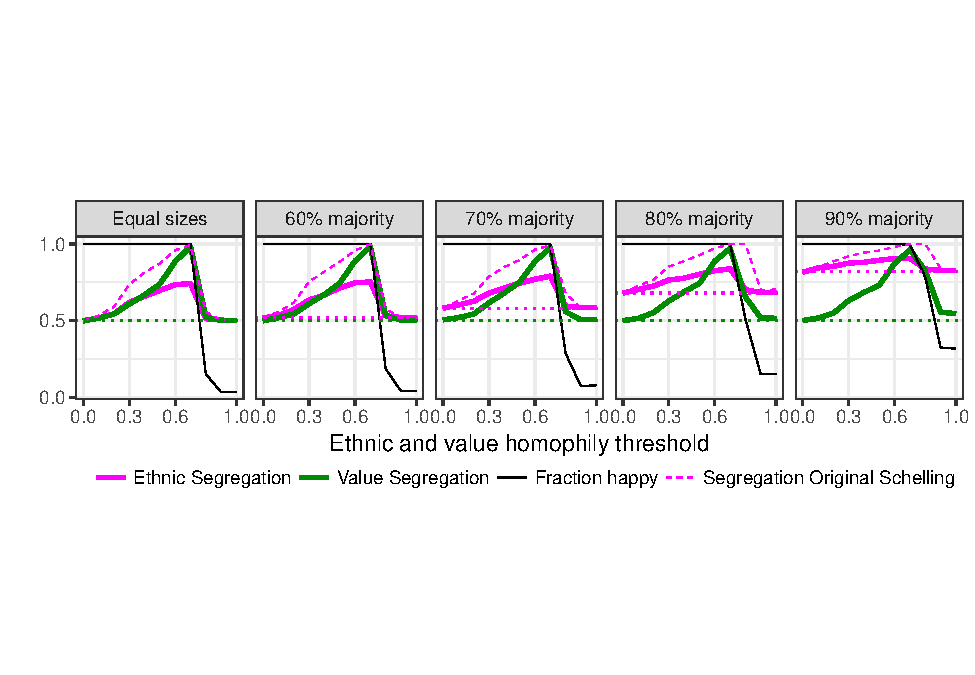
\psfig{file=OverallSegregation.eps,width=4.2cm}}
\vspace*{8pt}
\caption{Overall average local ethnic and value segregation for equal ethnic and value thresholds of ethnicity-oriented and value-oriented. In general the level of segregation is slightly lower than in Schelling's (1971)  original model. For thresholds above 0.5 local value similarity excels ethnic similarity.} 
\label{fig:OverallSegregation}
\end{figure}

The heatmap in Fig.~\ref{fig:Heatmap} includes both value-oriented and ethnicity-oriented agents for the {\it 50/50 society} and {\it 80/20 society} condition. The upper plots show that under parameter configurations with $\theta^\text{E} \leq 0.7$ and $\theta^\text{V} \leq 0.5$ happiness for all agents emerges. Interestingly, convergence to happiness is possible also for all of the value similarity thresholds, even the highest, when the ethnic similarity threshold is $\theta^\text{E} = 0.6$. Thus, even with  $\theta^\text{V} = 1$ the value-oriented half of the population can find a homogeneous neighborhood. The interesting point is that this would not be possible when the other, ethnicity-orientated half of the population would have a lower ethnic similarity threshold. Further on, the figure shows that value segregation can also be very high for moderate value similarity thresholds $0.4 \leq \theta^\text{V} \leq 0.5$ when the ethnic similarity threshold is very high $\theta^\text{E} \geq 0.8$. The effects are similar in the 50/50 and the 80/20 society with ethnic segregation being naturally a bit higher in the 80/20 society. 

\begin{figure}[th]
\centerline{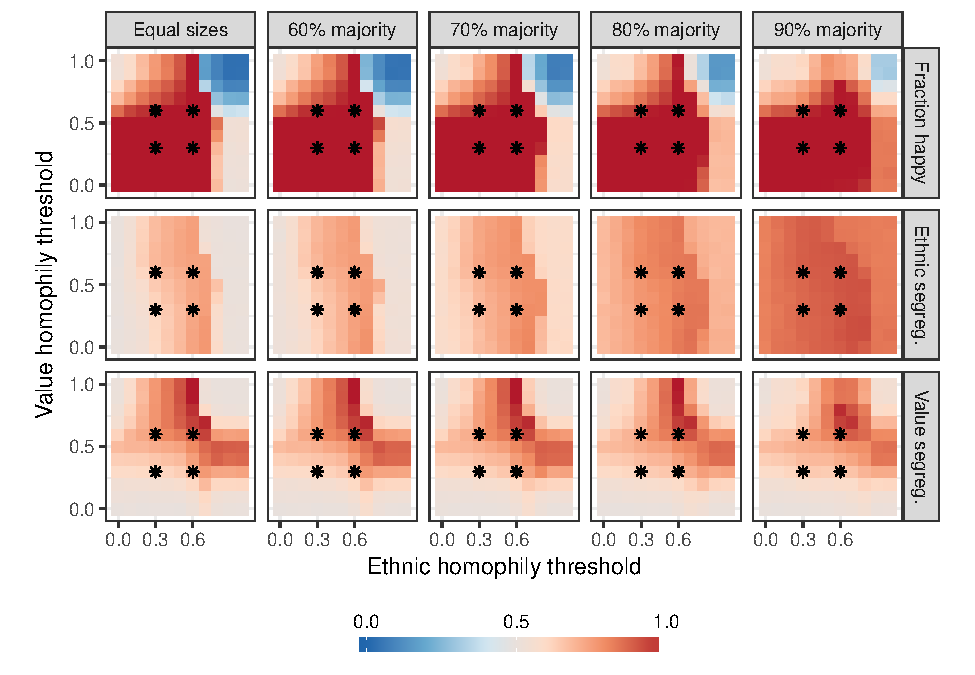
\psfig{file=Heatmap.eps,width=4.2cm}}
\vspace*{8pt}
\caption{Heatmap of average model outcomes for the fraction of finally happy agents, ethnic similarity, and value similarity. Similarity is measured as an average of the the fraction of neighbors which have the same ethnicity/value over all agents. High similarity is the same as high segregation.}
\label{fig:Heatmap}
\end{figure}

In Fig.~\ref{fig:Detail1} we want to focus on how a change of the ethnic similarity threshold $\theta^\text{E}$ affects value segregation $\Theta^\text{V}$. This is shown on the right-hand side of the figure. For moderate and higher value similarity thresholds $\theta^\text{V}=0.3$ or 0.7, value segregation increases with the increment of  ethnicity orientation. This happens in particular for the minority group in the 80/20 society. 


\begin{figure}[th]
\centerline{\psfig{file=Detail1.eps,width=4.2cm}}
\vspace*{8pt}
\caption{The effect of the ethnic similarity threshold. Ethnic (left) and value (right) segregation as a function of the ethnic similarity threshold for three values of the value similarity threshold (0, 0.3 and 0.7). Each subplot goes along a horizontal line in the.}
\label{fig:Detail1}
\end{figure}

In Fig.~\ref{fig:Detail2} we focus the other way round on how a change of the value similarity threshold $\theta^\text{V}$ affects ethnic segregation $\Theta^\text{E}$. This is shown on the left-hand side of the figure. Effects appear more evident for a moderate ethnic similarity threshold $\theta^\text{E} = 0.3$. In this case, an increasing value-orientation increases ethnic segregation but only for the ethnicity-oriented agents. For the value-oriented agents even a very mild decrease of ethnic segregation can be observed. For moderate and higher ethnicity similarity thresholds $\theta^\text{E}=0.3$ or 0.7, ethnic segregation increases with increasing value orientation. This happens in particular for the minority group in the 80/20 society.

\begin{figure}[th]
\centerline{\psfig{file=Detail2.eps,width=4.2cm}}
\vspace*{8pt}
\caption{The effect of the value similarity threshold. Ethnic (left) and value (right) segregation as a function of the value similarity threshold for three values of the ethnic similarity threshold (0, 0.3 and 0.7). Each subplot goes along a vertical line in the.}
\label{fig:Detail2}
\end{figure}

Finally, we show in Fig.~\ref{fig:Densities} the average local densities of subgroups and how they depend on the ethnic similarity threshold for different value similarity thresholds. In the 50/50 society and a moderate or high value similarity threshold $\theta^\text{V}=0.3$ or 0.7, a general trend is that value-oriented agents usually live in denser regions. This can be a tendency of tolerance-orientation agents to live in urban regions, while ethnicity-orientated agents tend to live in rural regions. Interesting phenomena appear in the 80/20 society with strong value-orientation $\theta^\text{V}=0.7$. For moderate ethnicity-orientation only the ethnicity-oriented from the majority ethnicity tend to live in rural regions while the ethnicity-oriented minority ethnicity also live in more urban regions, which reverses for stronger ethnicity orientation. 

\begin{figure}[th]
\centerline{\psfig{file=Densities.eps,width=4.2cm}}
\vspace*{8pt}
\caption{Density study for subgroups along a horizontal lines in the coneptual for value similarity thresholds 0, 0.3, and 0.7.}
\label{fig:Densities}
\end{figure}

We can provide some explanation for the results of our simulations based on the combined effect of the group sizes and the two diverse criteria of similarity introduced in agents. As shown in Fig.~\ref{fig:Modelconditions}, since half of the population is ethnicity-oriented and half is value-oriented, no matter the equal size or majority/minority condition, value-oriented agents do always represent half of the total population. This allows them to have 0.5 probability to relocate close to other similar value-oriented agents, explaining their tendency to live in denser and more robust neighborhoods where ethnic segregation is mitigated when agents belong to diverse ethnicities. Consequently, ethnicity-oriented agents find attractive those neighborhoods where value-oriented agents of the same ethnicity have relocated, thus consequently increasing the ethnic segregation of the same neighborhood. Nevertheless, all agents can be happy only for some combinations of ethnic threshold $\theta^\text{E}$ and value threshold $\theta^\text{V}$ as shown in Fig.~\ref{fig:Heatmap}. Ethnicity-oriented majority agents have 0.8 probability to find agents of the same ethnicity, so to be less sensitive to the presence of agents of the other ethnicity. Moreover, due to the high probability they can spread more sparsely in the world, explaining why they appear more in rural areas. On the contrary, ethnicity-oriented minority agents have a lower 0.2 probability to relocate close to similar agents of the same ethnicity, which explains why they relocate more easily in their neighborhoods, but at the same time they are more sensitive to the ethnical diversity of the neighborhood due to the numerical minority. Thus, we can conclude that there is a spillover effect where value segregation in our simulations is likely to spur ethnic segregation under some conditions, namely in the condition of minority, whereas the contrary cannot hold.

\begin{figure}[th]
\centerline{\psfig{file=Modelconditions.eps,width=4.2cm}}
\vspace*{8pt}
\caption{Theoretical model in the 50/50 society and the 80/20 society conditions.}
\label{fig:Modelconditions}
\end{figure}

\section{Conclusion and Discussion}

Our model can provide some insights for real societies, showing how value segregation and ethnic segregation that seem potentially opposite could not be necessarily independent, but coexist and even be interdependent. As our simulation suggests, in multicultural and more diverse societies as of today, people who show more tolerance towards diversity and highlight shared values and characteristics are more likely to adapt to any residential option and contribute to cohesiveness of integrated societies. But as our model shows, this can  generate what we observe in our simulation as a spillover effect from value to ethnic segregation. People not willing to integrate and fostering segregation between groups (as ethnic-oriented agents in our simulation), might paradoxically find attractive those ethnically diverse neighborhoods where a certain fraction of tolerant people of the same ethnicity resides in, so to attract consequently other ethnic-oriented people and increase  the ethnic segregation of the area. This would demonstrate that ethnic diversity or segregation of a neighborhood might not necessarily be the direct effect of attitudes against a group, but the emerging result of overlapping individual preferences.

Our model might have some other applications based on the spillover effect it shows. Although we focus on a homophily behavior and not on devaluing of the other group, the emergent effect we observe in our simulations could apply to more drastic phenomena as political intolerance and social turmoil against migrant acceptance. Ethnic-oriented agents in our simulation are more likely to share such attitudes, which might increase due to spatial proximity as in models of assimilative social influence \cite{flache2017}. As our model demonstrates, their clustering could happen not only in ethnically segregated neighborhoods that intolerant ones form, but under some conditions also in ethnically integrated neighborhoods formed by tolerant ones driven by value-orientation. In this case, a cascade emerges from the behavior of tolerant agents, whose neighborhoods can become attractive to intolerant ones due to members of the own ethnic group. Intolerant newcomers would then be initially accepted as their presence is not a threat to the value composition of tolerant neighborhoods, but with the risk to attract eventually more ethnicity-oriented intolerant and so increase the ethnic segregation of such neighborhoods. In such a scenario, consensus towards intolerance in the neighborhood might emerge not as an effect of political attitude of intolerant people, but from the mutual adaptation of other residential choices involving both intolerant and tolerant subpopulations

\bibliographystyle{ws-acs}
\bibliography{ws-acs}

\end{document}